\documentclass{sig-alternate}

\usepackage{graphicx}
\usepackage{listings}
\usepackage{url}
\usepackage{hyperref}
\hypersetup{breaklinks}

\begin{document}
\title{Homework 1: Local Search}
\author{Ross Nordstrom\\
        University of Colorado - Colorado Springs\\
        1420 Austin Bluffs Pkwy,\\
        Colorado Springs, CO 80918\\
        \texttt{rnordstr@uccs.edu, nordstrom.ross@gmail.com}
       }
\date{March 11, 2015}

\maketitle

\begin{abstract}
   This paper presents a solution to a home work assignment using the N-Queens problem to drive
   an understanding of local search. The solution presented here is built in AngularJS, complete
   with a UI and complete parametrization, single step evaluation, and a debug view to help
   teach how N-Queens and hill climbing work. The results are best viewed live by running
   the accompanying code suite in a browser, with installation instructions in the README.md file.
\end{abstract}

\category{I.2.8}{Problem Solving, Control Methods, and Search}{Heuristic methods}
\terms{Machine Learning}
\keywords{Machine Learning, Artificial Intelligence, N-Queens, Local Search, Hill Climbing}

\section{Implementation}
\label{section:implementation}
The N-Queens hill climbing solution presented in this paper was implemented in AngularJS, in order to more easily
develop the solution, and quickly prototype a UI built for exploring the problem. The solution presented here is an
excellent source for learning Hill Climbing because of certain extensions made to the original assignment, and the
focus on interaction.

\subsection{Application Structure}
The application itself is stored as AngularJS code served by a Node.js API. The project is built with modern practices,
so \texttt{package.json} describes the Node.js dependencies and project configuration and \texttt{bower.json} describes
the client-side dependencies.

\subsubsection{Setup}
To run the project, the following must be installed on the machine:
\texttt{node}\cite{node}, \texttt{npm}\cite{npm}, \texttt{bower}\cite{bower}.

Then use \texttt{npm} and \texttt{bower} to install the dependencies:

\begin{lstlisting}
# Install server dependencies
npm install

# Install client JS dependencies
bower install
\end{lstlisting}

\subsubsection{Running}
The project is setup to run easily, using scripts defined in \texttt{package.json}. Simply run the following:

\begin{lstlisting}
npm start
\end{lstlisting}

Then browse to the page at \url{http://localhost:8080}

\subsubsection{Javascript Files}
The core of the project is in the Javascript files under \texttt{n-queens/public/js}. Here, each folder and file within
is described:

\begin{description}
  \item[/controllers]   -- Contains business logic wiring up Hill Climbing backend code to user interaction in the UI
  \begin{description}
    \item{BruteCtrl.js} -- Manages the brute force page
    \item{ClimbCtrl.js} -- Manages the Hill Climbing page
    \item{MainCtrl.js}  -- Not used
  \end{description}
  \item[/filters]       -- Contains AngularJS filters, which help transform data/text in the UI
  \item[/services]      -- Contains models and core code implementing the Hill Climbing algorithms
  \item[app.js]         -- Declares the AngularJS application, including dependencies
  \item[appRoutes.js]   -- Defines the app routes, connecting URLs to a controller and view
\end{description}

\section{Results}
\label{section:results}
Here, approaches taken and results found are presented for each of the questions in the assignment. Evaluations were
made against a single randomly generated board in order to consistently compare their success. A side effect of this
is that some evaluations on better boards were highly successful, while worse boards were much less successful.

\subsection{Basic Hill Climbing}
By specifying a number of ``times'' in the evaluation configuration, the application will try to do hill climbing that
many times on a randomly generated board each time. In 1000 runs, the success rate was 18.9%, with the successful runs
succeeding in a mean of 5 steps (min: 3, max: 8), taking a mean of 36.3ms (min: 8.0ms, max: 60.0ms). Of the 1000 runs,
485 of the failures ended with 1 pair of attacking queens, 257 ended with 2 pairs of attacking queens, and 38 ended with
3 pairs of attacking queens.

\subsection{Hill Climbing with K Sideways Moves}
Introducing sideways moves seems to have a delayed improvement on the success rate, where 2-3 sideways moves hurts the
success rate, but more moves improves it, over the base of 0 sideways moves allowed \ref{sideways}

\begin{figure}[ht!]
\centering
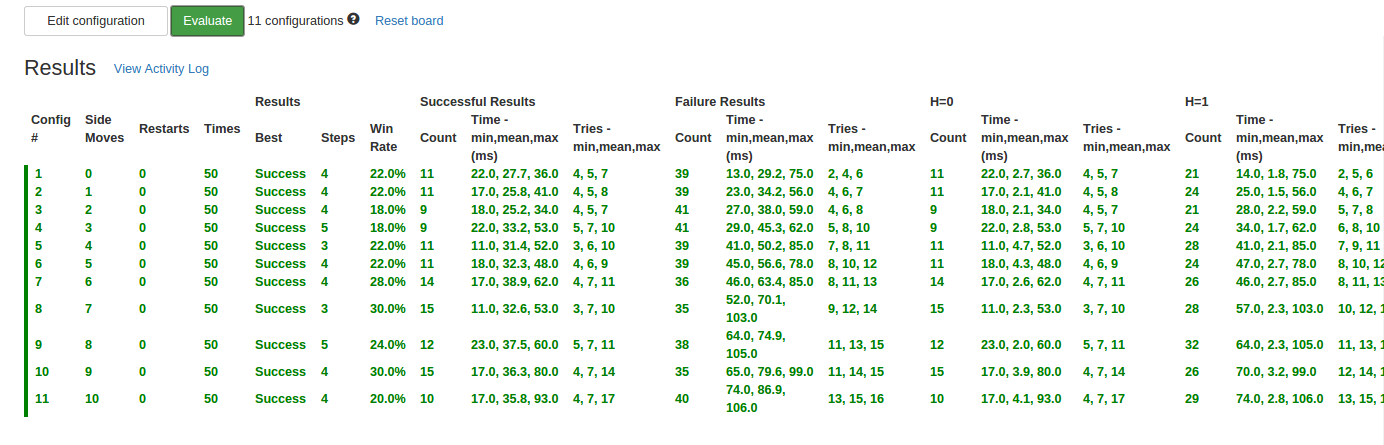
\includegraphics[width=90mm]{img/sideways.png}
\caption{Results showing win rates with sidways moves in the range k=[0:10]. Improvements are not realized until k=6}
\label{fig:ui}
\end{figure}


\subsection{Hill Climbing with Random Restarts}


\subsection{Hill Climbing with Sideways Moves and Random Restarts}


\subsection{Extension: Brute Force via Random Generation}


\section{Future Work}
\label{section:futurework}
While all of the required goals were met, future work could improve upon the application by optimizing board modelling
and manipulation through maintining a single array of queen information rather than a 2D representation of the board
with queen state stored withing. This would improve on both storage and -- more so -- on computation times.

Additionally, future work could include visualization of the algorithm's success, making it easier to understand.

\bibliography{citations}{}
\bibliographystyle{plain}

\end{document}
